\section{Le trognon d'un langage}

\subsection{Définition}

\setframetitle{Définition}

\begin{frame}{\myframetitle}
  \begin{block}{Le trognon d'un mot}
    \centering
    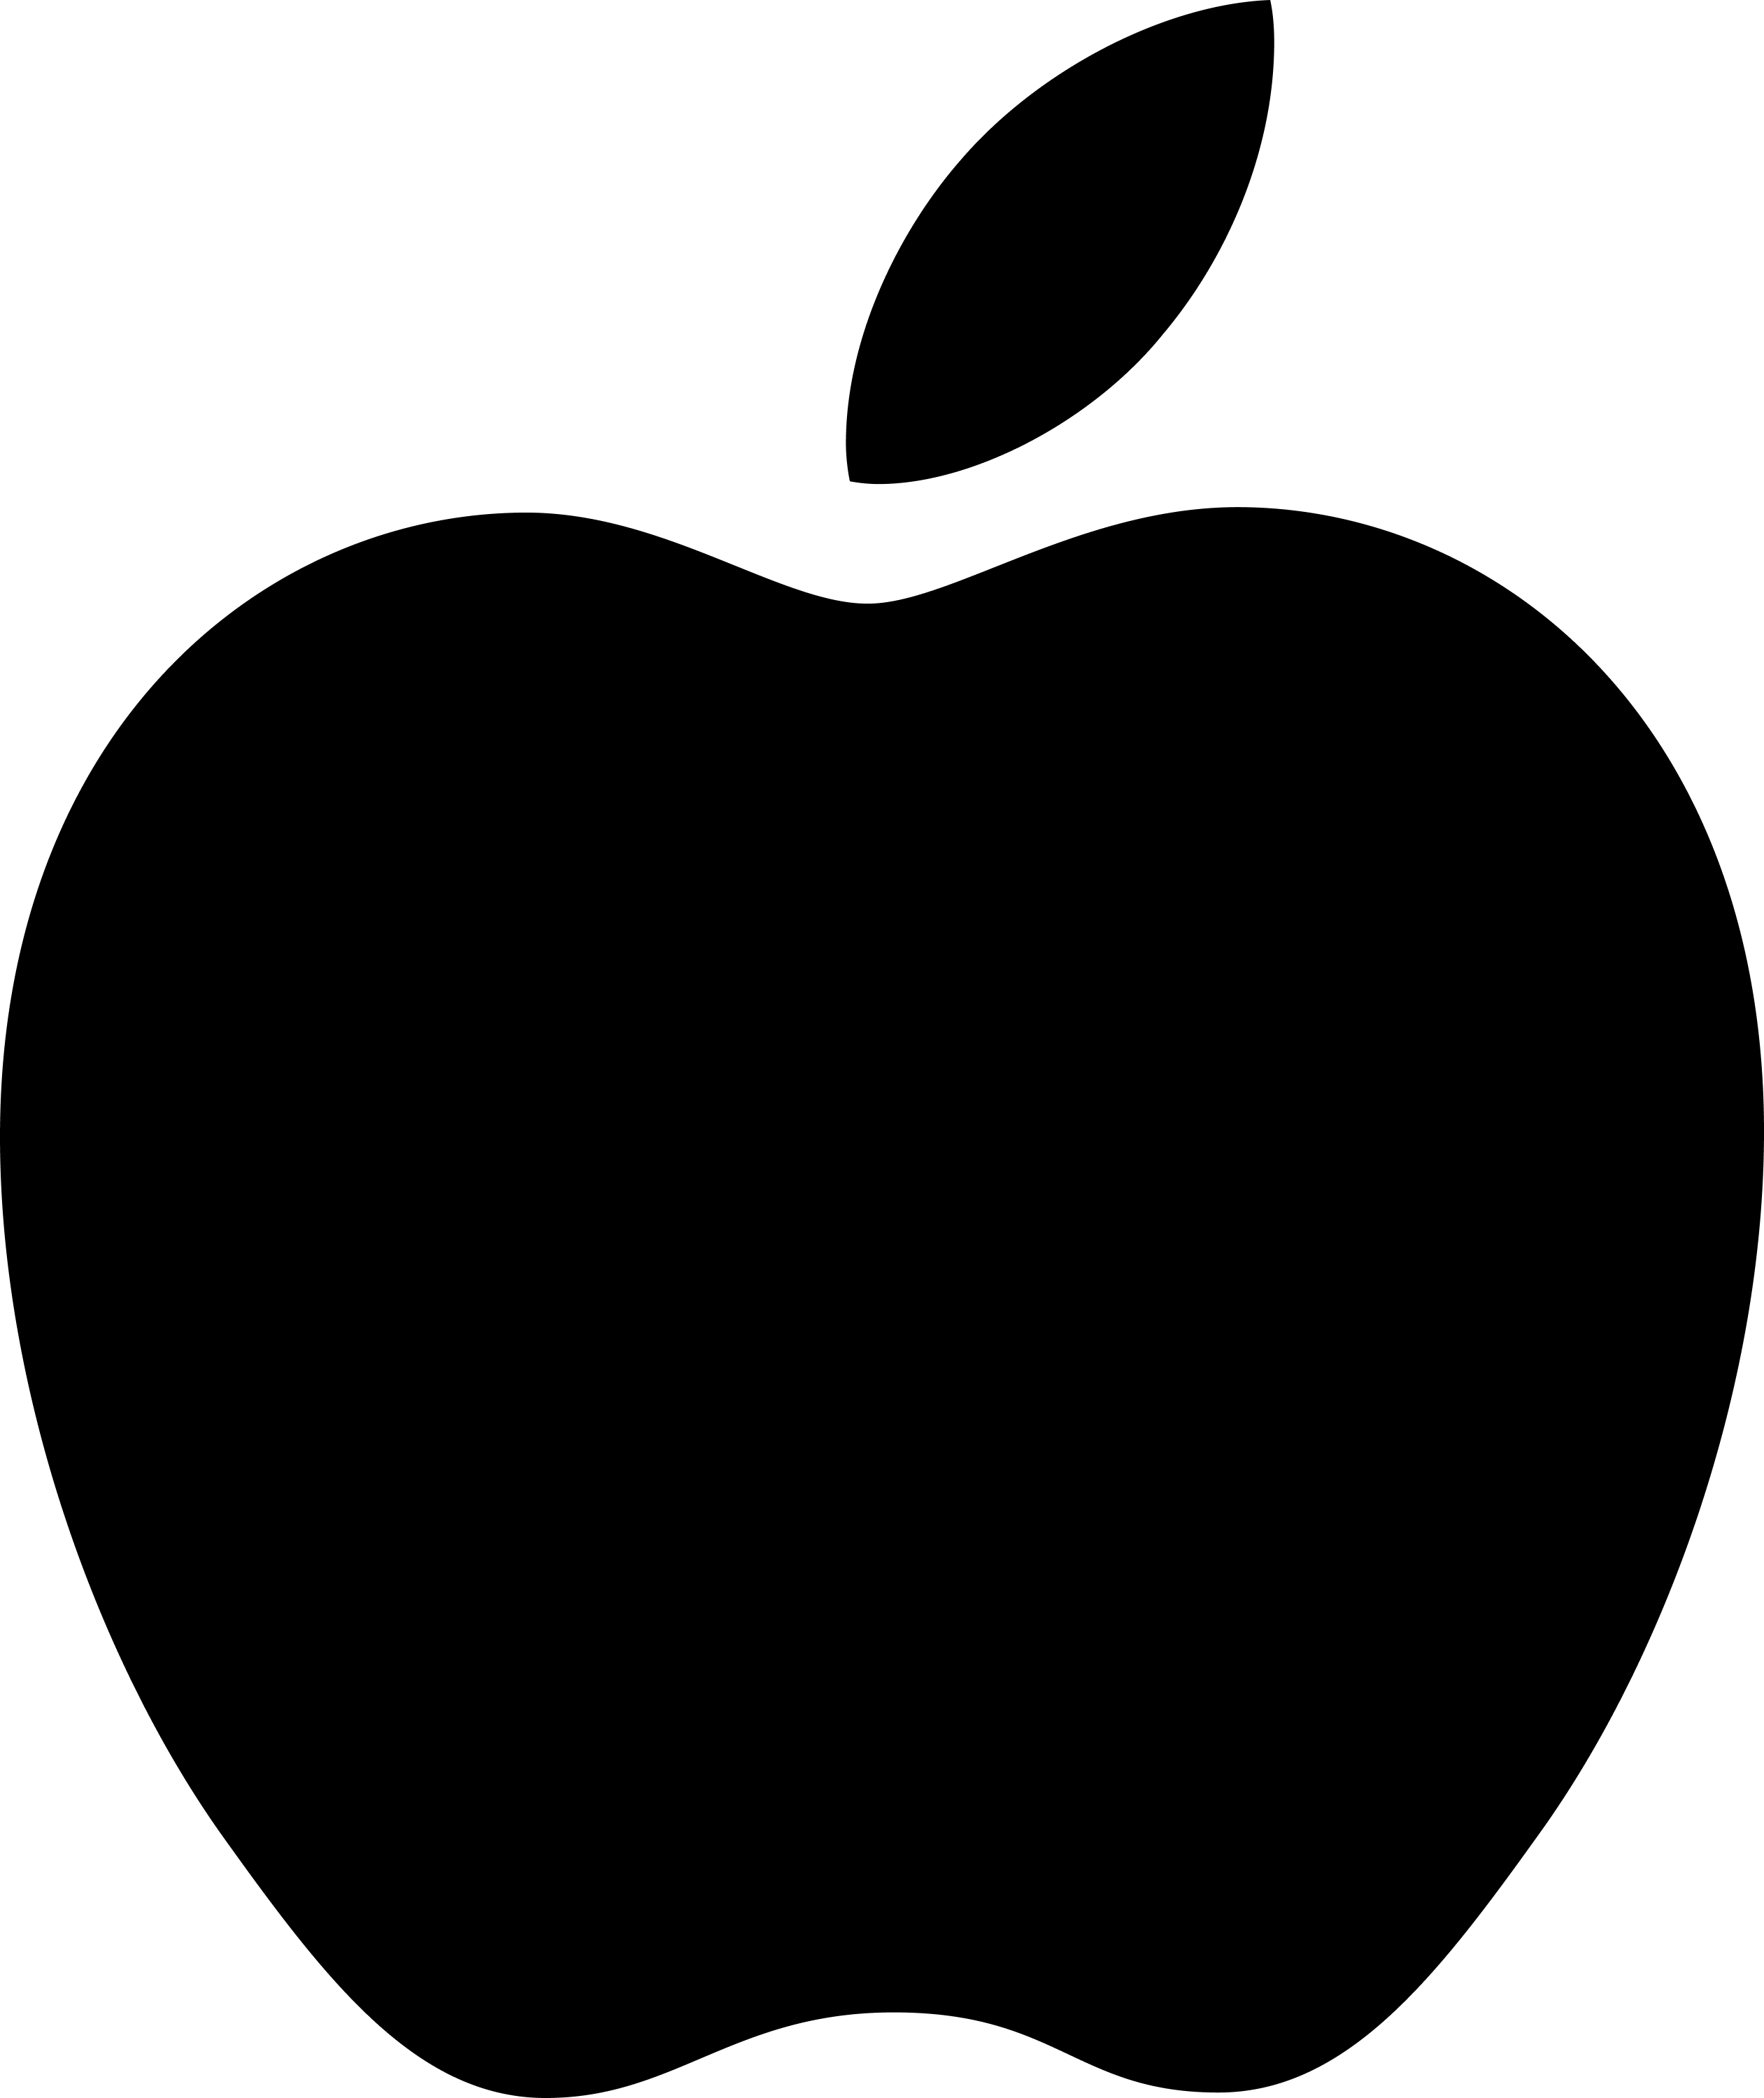
\includegraphics[width=0.25\textwidth]{./resources/full_apple.png}

    \pause[]

    \vphantom{}

    \Large{\(abcdcba\)}
  \end{block}
\end{frame}

\begin{frame}{\myframetitle}
  \begin{block}{Le trognon d'un mot}
    \centering
    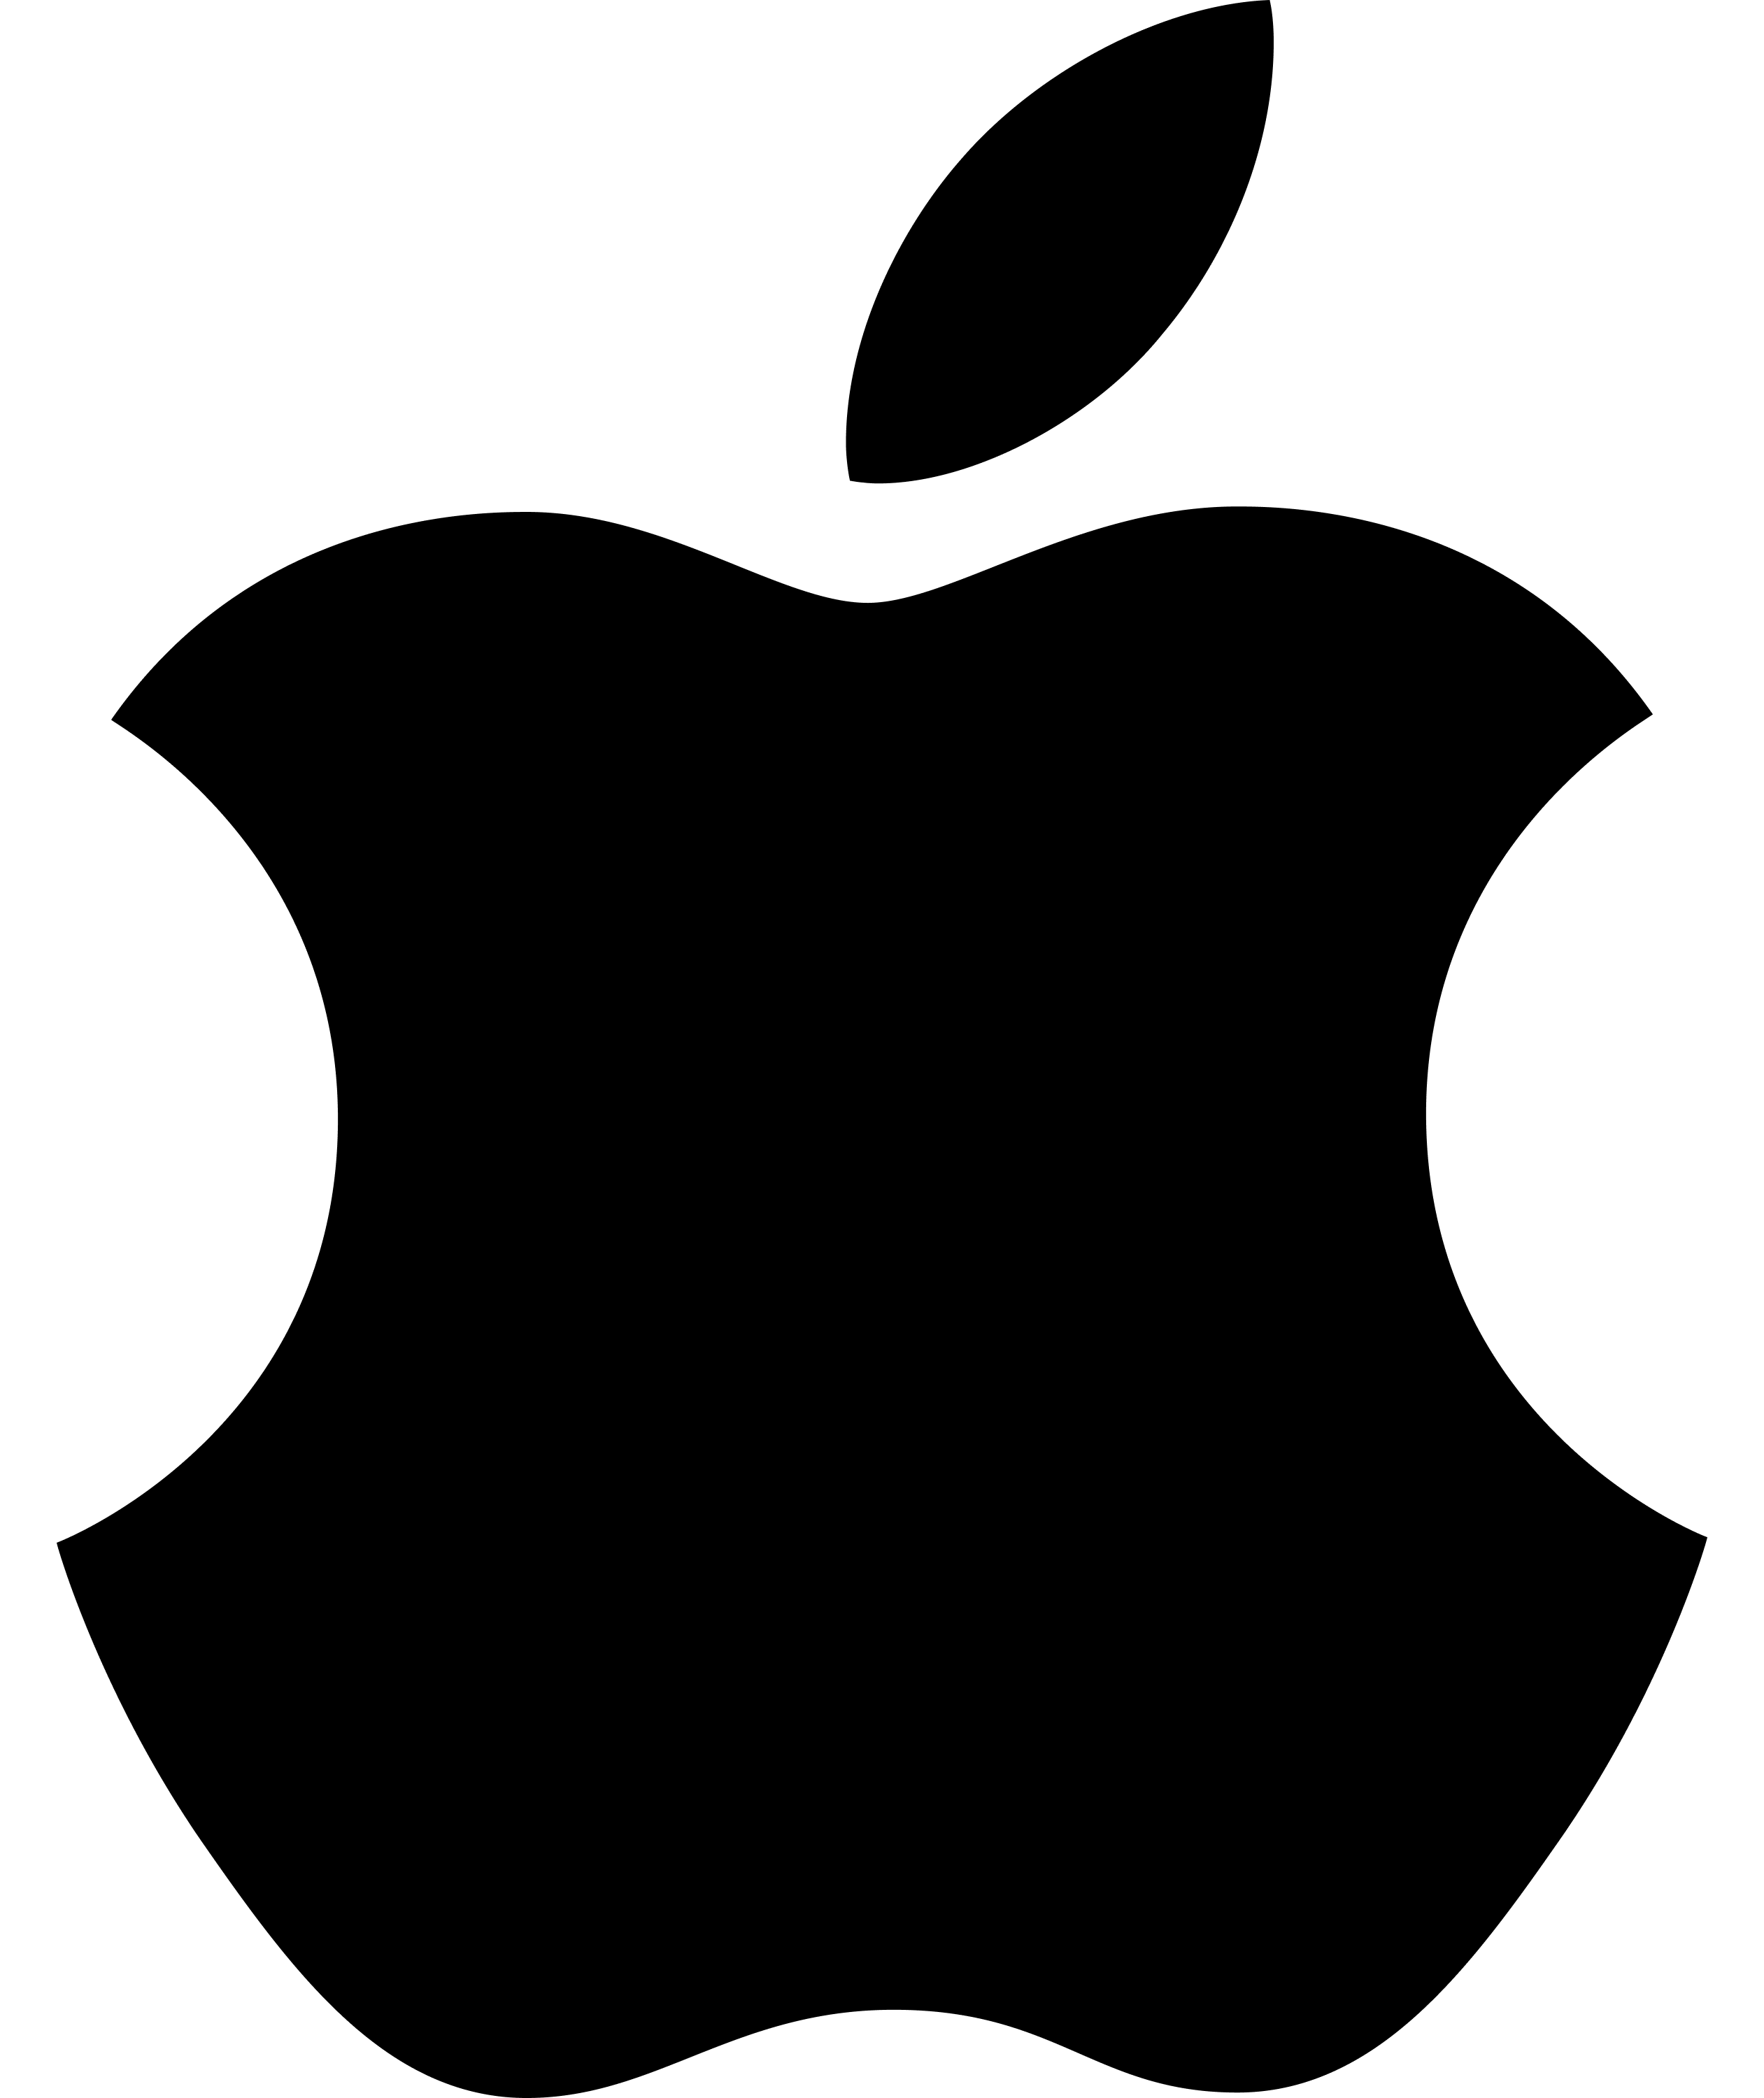
\includegraphics[width=0.25\textwidth]{./resources/mid_apple.png}

    \pause[]

    \vphantom{}

    \Large{\(\color{red}{ab} \color{black}{\cdot cdc \cdot} \color{red}{ba}\)}
  \end{block}
\end{frame}

\begin{frame}{\myframetitle}
  \begin{block}{Le trognon d'un mot}
    \centering
    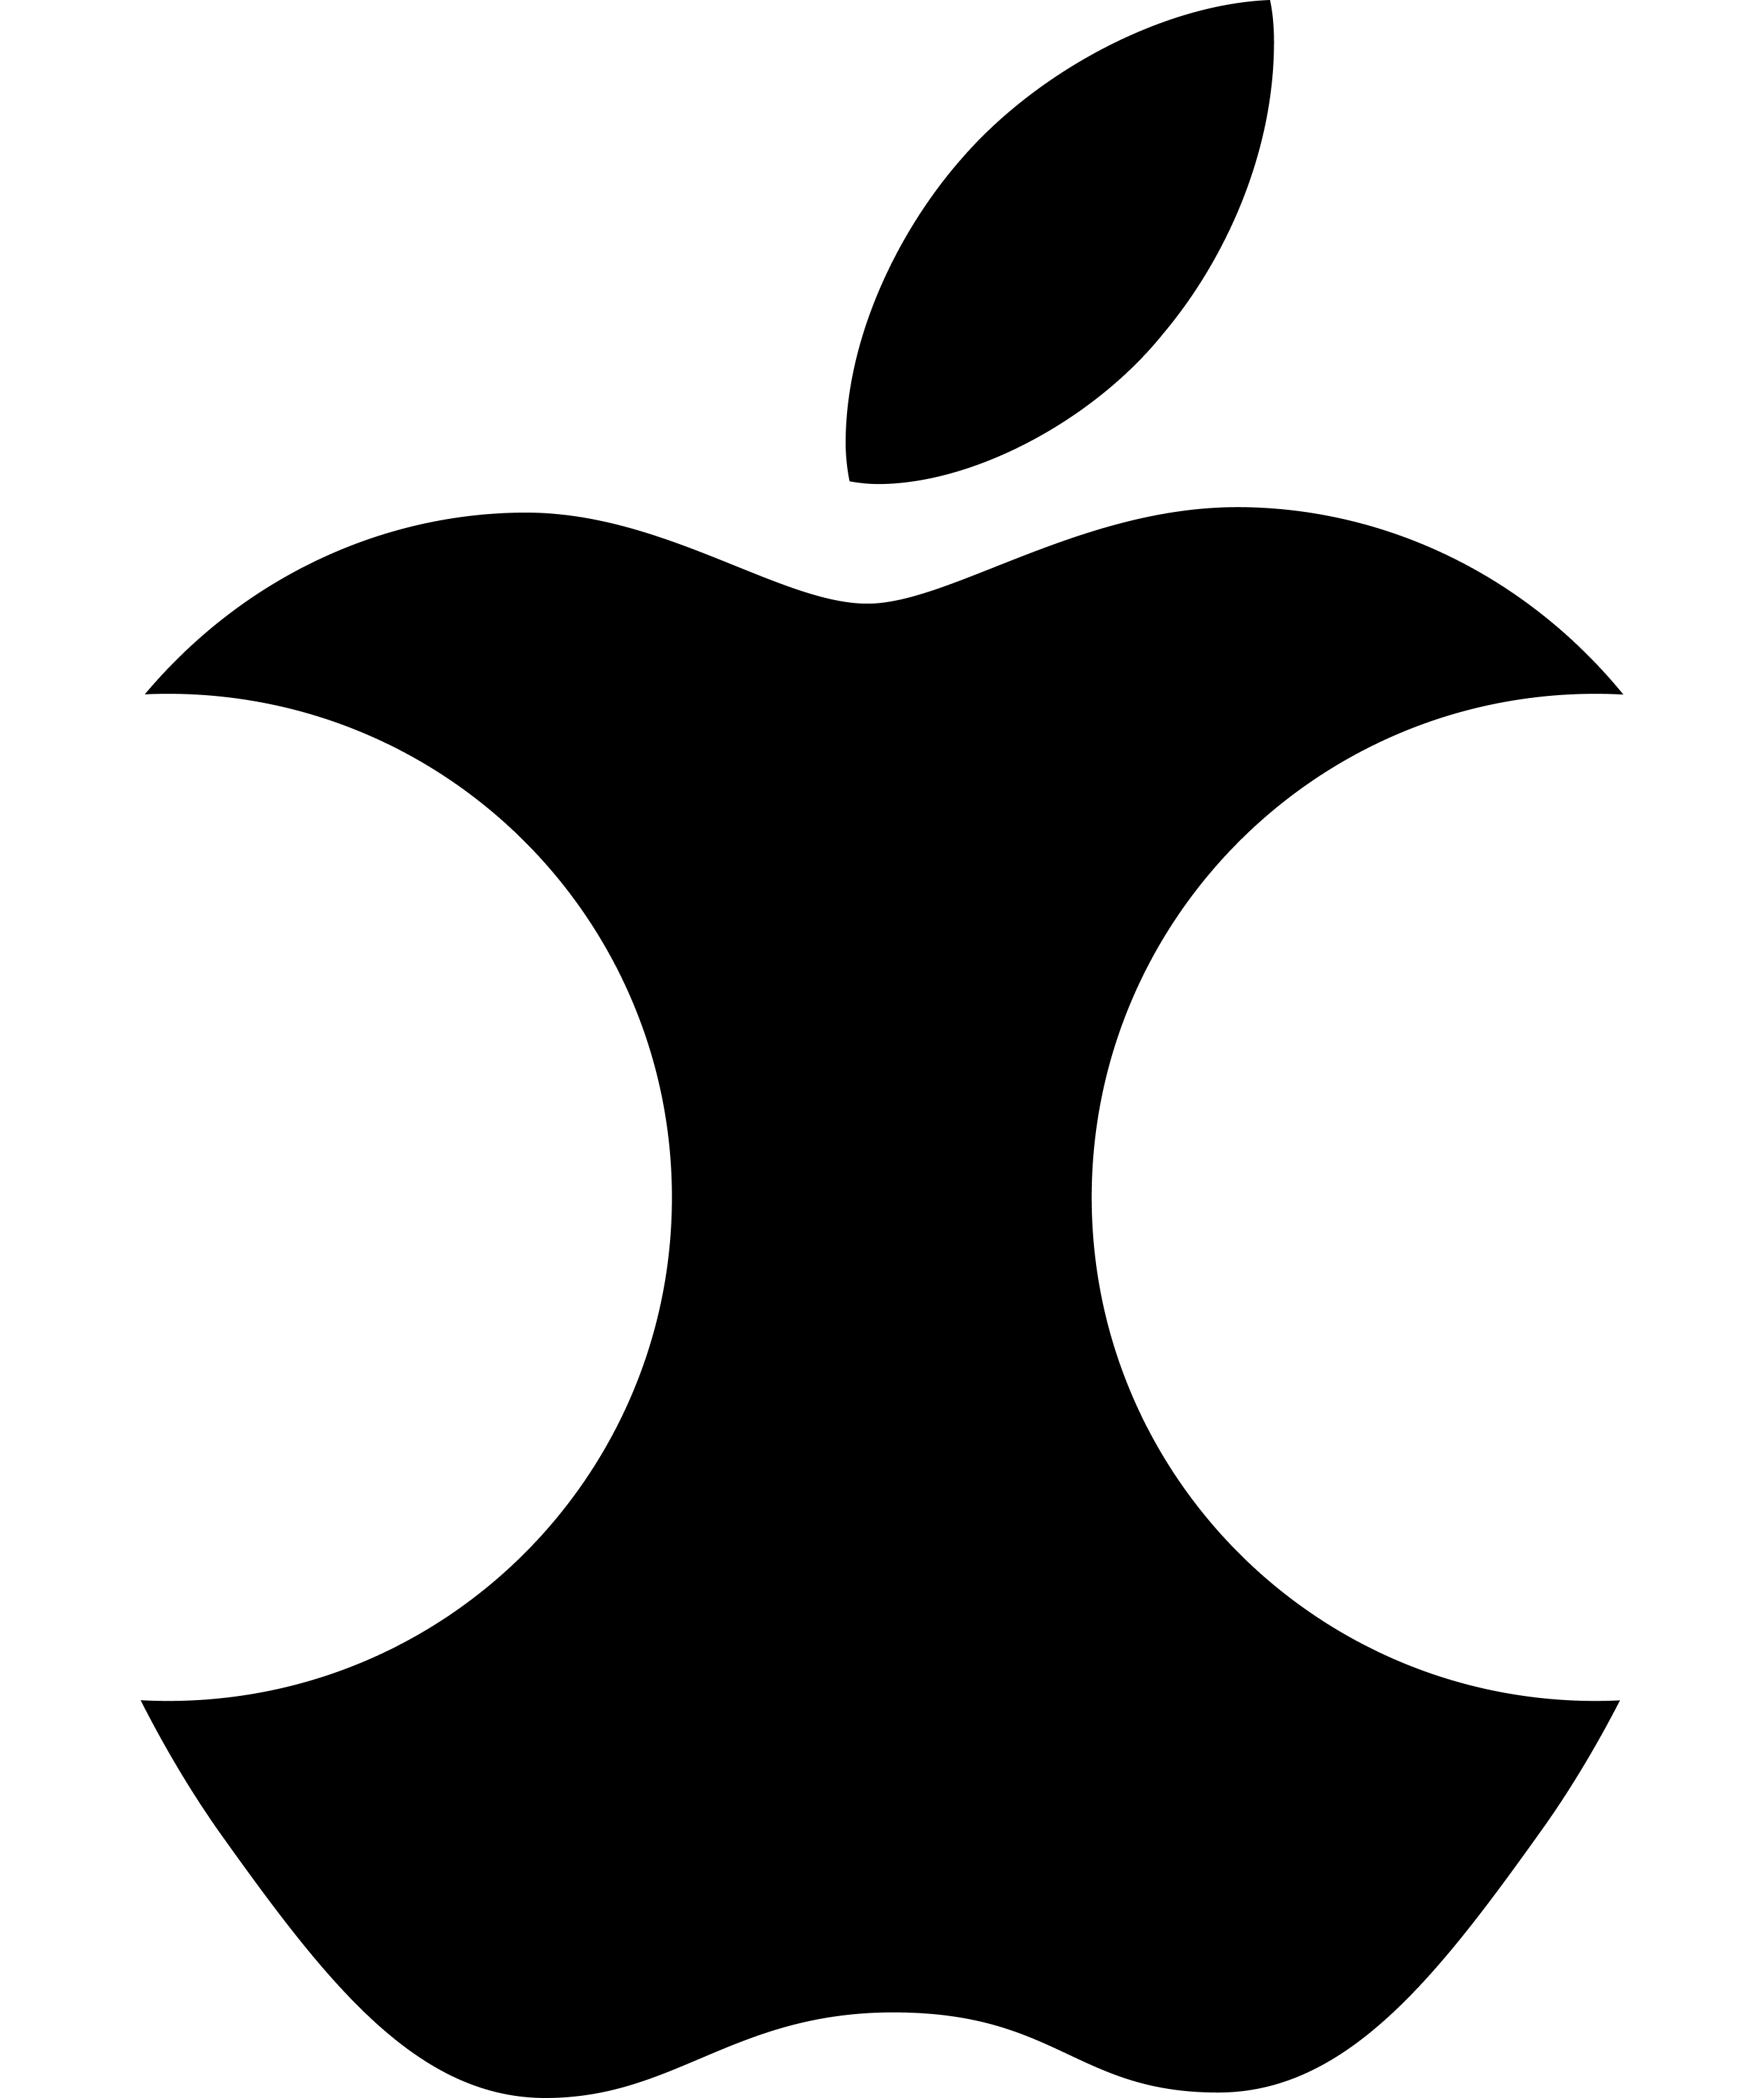
\includegraphics[width=0.25\textwidth]{./resources/empty_apple.png}

    \pause[]

    \vphantom{}

    \Large{\(\color{red}{abc} \color{black}{\cdot d \cdot} \color{red}{cba}\)}
  \end{block}
\end{frame}

\begin{frame}{\myframetitle}
  \begin{block}{Le trognon d'un mot}
    \centering
    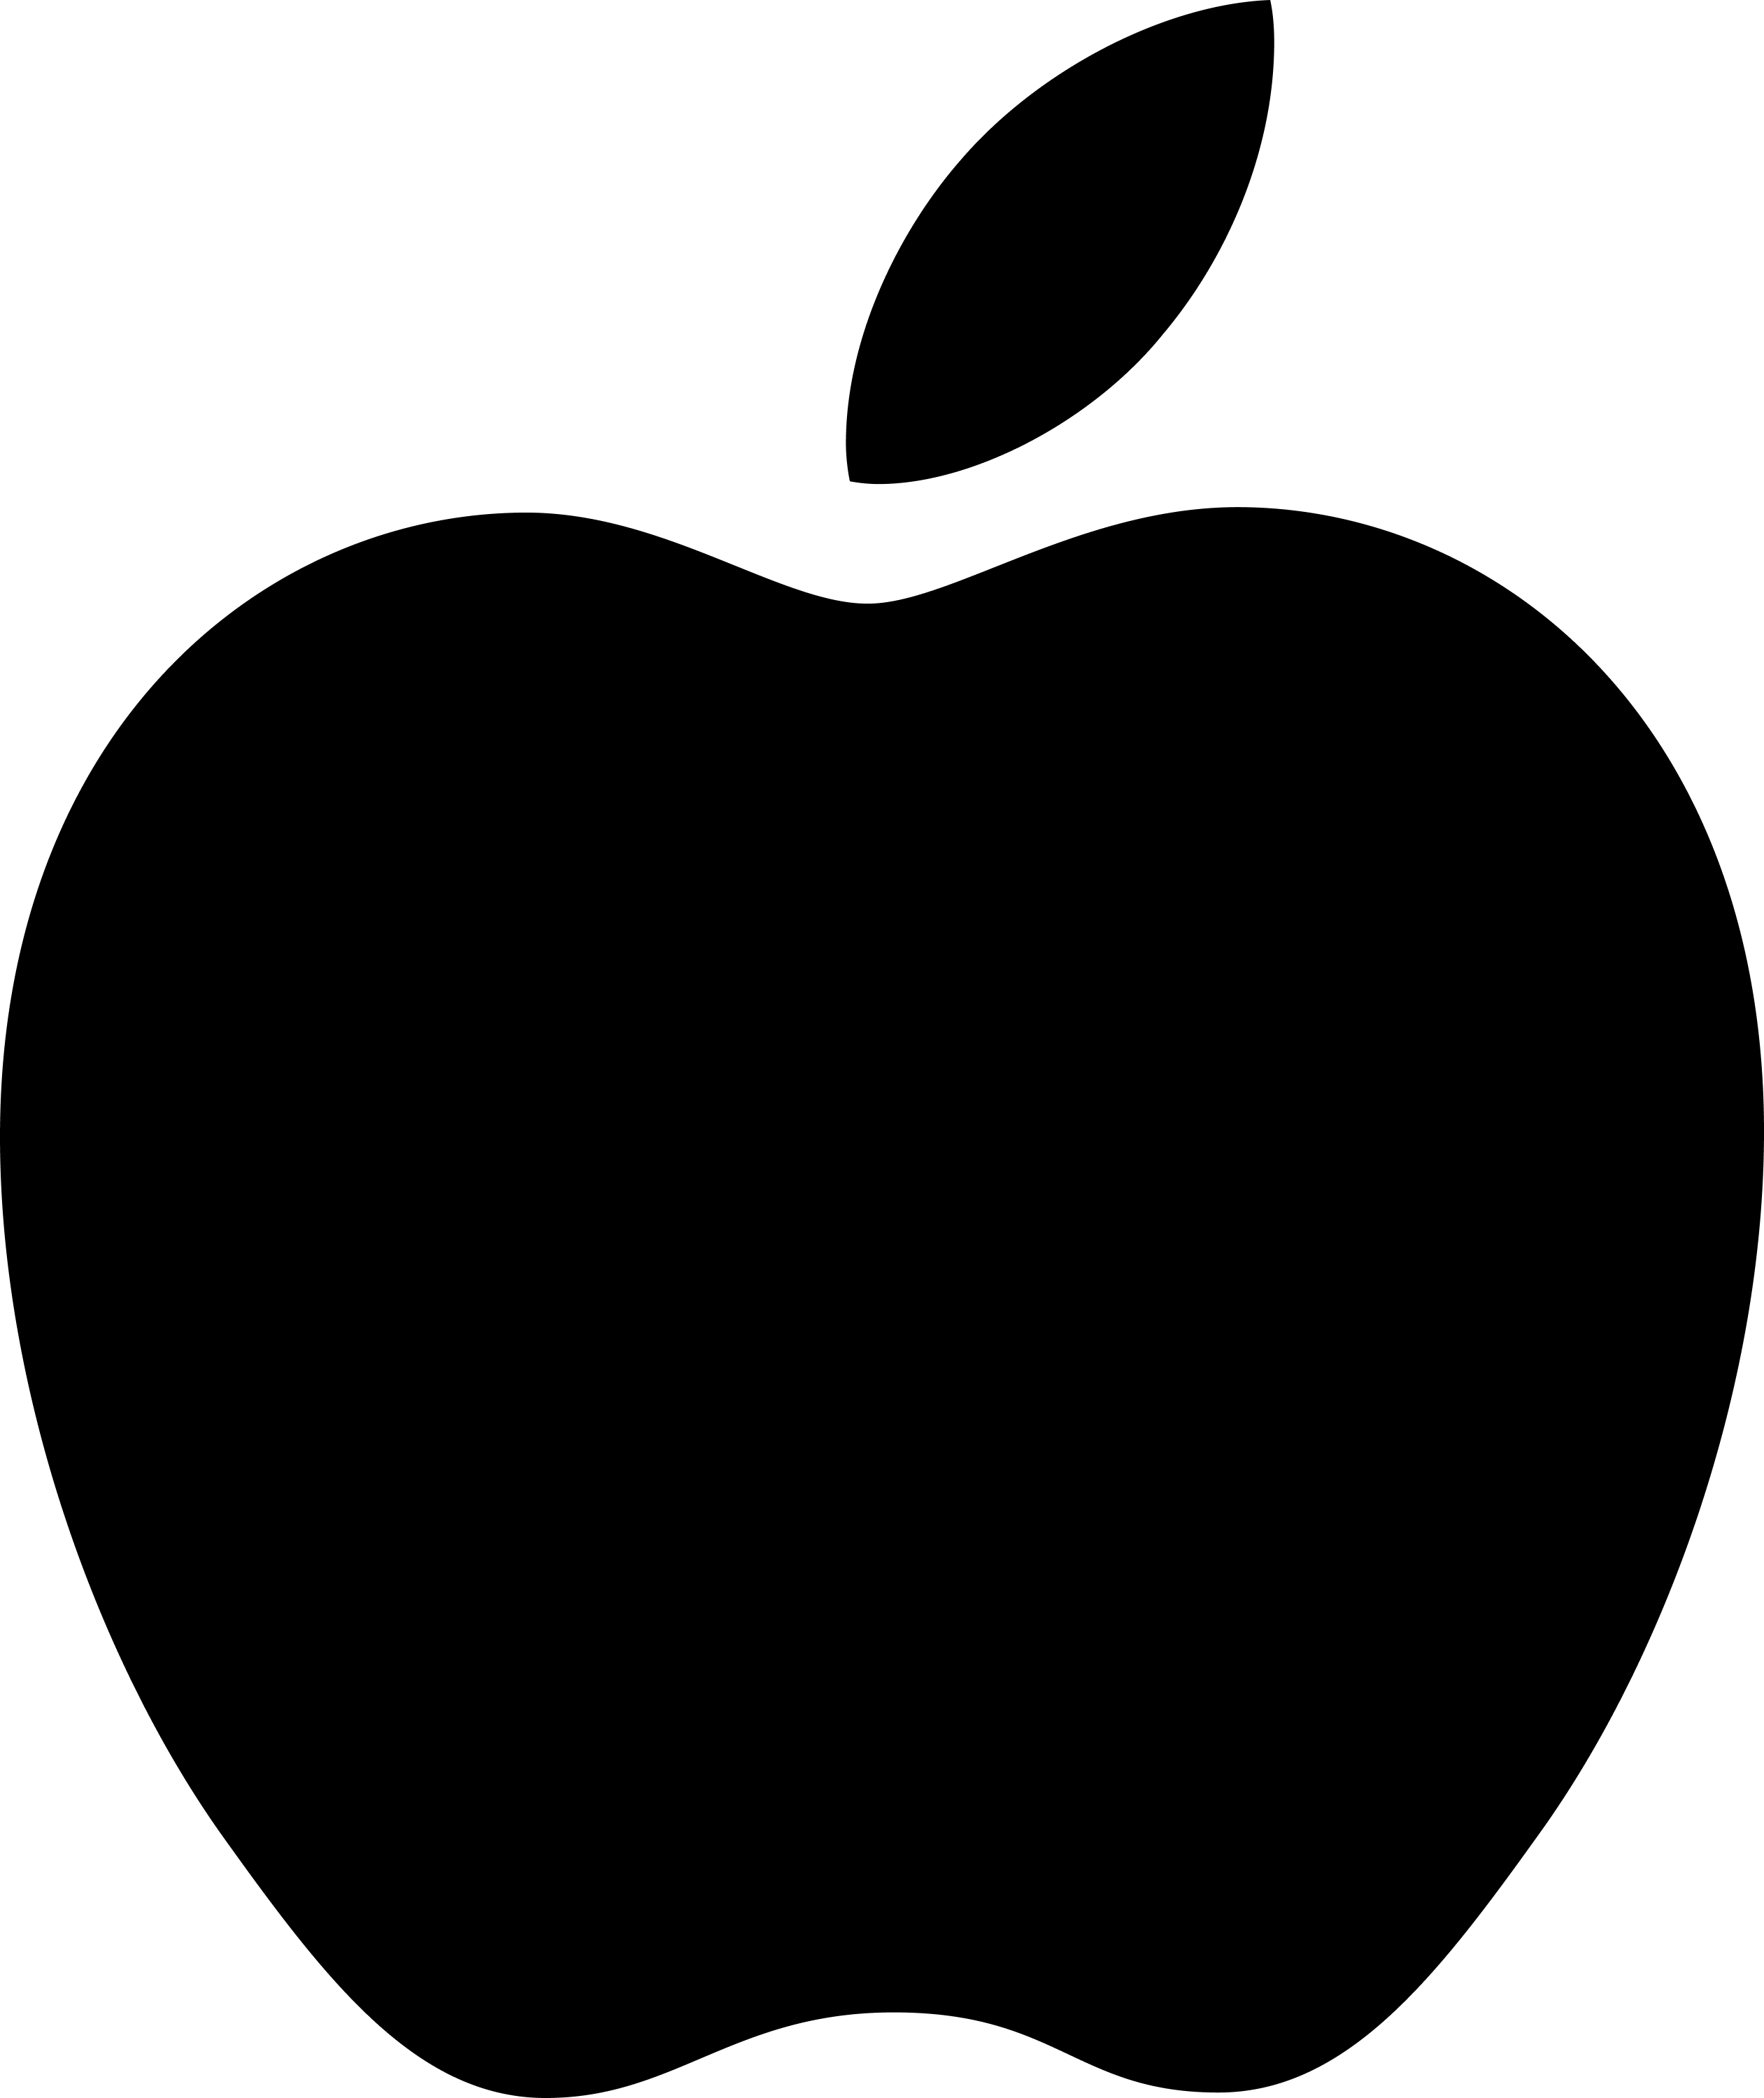
\includegraphics[width=0.25\textwidth]{./resources/full_apple.png}

    \pause[]

    \vphantom{}

    \Large{\(\color{red}{\varepsilon} \color{black}{\cdot abcdcba \cdot}
    \color{red}{\varepsilon}\)}
  \end{block}
\end{frame}

\begin{frame}{\myframetitle}
  \begin{definition}[Le trognon d'un mot]
    Le trognon d'un langage sera alors l'union des trognons des mots qu'il le
    compose.
  \end{definition}
\end{frame}

\subsection{Algorithme de grignotage}

\setframetitle{Algorithme de grignotage}

\begin{frame}{\myframetitle}
  \begin{example}[\(L(M) = a \cdot a^* \cdot c \cdot a^* \cdot a\)]
    \begin{center}
      \begin{tikzpicture}
        \node[state, initial] (1) {\(1\)};
        \node[state, right of=1] (2) {\(2\)};
        \node[state, right of=2] (3) {\(3\)};
        \node[state, accepting, right of=3] (4) {\(4\)};

        \draw
        (1) edge[above] node{\(a\)} (2)
        (2) edge[loop above] node{\(a\)} (2)
        (2) edge[above] node{\(c\)} (3)
        (3) edge[loop above] node{\(a\)} (3)
        (3) edge[above] node{\(a\)} (4);
      \end{tikzpicture}
    \end{center}
  \end{example}
\end{frame}

\begin{frame}{\myframetitle}
  \begin{example}[\(M\) grignoté de \(a\)]
    \begin{center}
      \begin{tikzpicture}
        \node[state] (1) {\(1\)};
        \node[state, initial below, right of=1] (2) {\(2\)};
        \node[state, accepting, right of=2] (3) {\(3\)};
        \node[state, right of=3] (4) {\(4\)};

        \draw
        (1) edge[above, red] node{\(a\)} (2)
        (2) edge[loop above] node{\(a\)} (2)
        (2) edge[above] node{\(c\)} (3)
        (3) edge[loop above] node{\(a\)} (3)
        (3) edge[above, red] node{\(a\)} (4);
      \end{tikzpicture}
    \end{center}
  \end{example}
\end{frame}

\begin{frame}{\myframetitle}
  \begin{example}[\(M\) grignoté de \(aa\)]
    \begin{center}
      \begin{tikzpicture}
        \node[state] (1) {\(1\)};
        \node[state, initial below, right of=1] (2) {\(2\)};
        \node[state, accepting, right of=2] (3) {\(3\)};
        \node[state, right of=3] (4) {\(4\)};

        \draw
        (1) edge[above, red] node{\(a\)} (2)
        (2) edge[loop above, red] node{\(a\)} (2)
        (2) edge[above] node{\(c\)} (3)
        (3) edge[loop above, red] node{\(a\)} (3)
        (3) edge[above, red] node{\(a\)} (4);
      \end{tikzpicture}
    \end{center}
  \end{example}
\end{frame}

\begin{frame}{\myframetitle}
  \begin{definition}
    L'automate \(\texttt{nibbling}(M)\) sera donc l'union des automates
    grignotés distincts.
  \end{definition}

  \pause[]

  \begin{block}{Compléxité en état de notre algorithme}
    Le nombre d'états de l'union de deux automates est égal à la somme des
    nombres d'états des automates.

    \pause[]

    \vphantom{}

    Les automates grignotés ont comme forme \((Q, I, F, \delta)\) avec \(Q\)
    et \(\delta\) les mêmes et comme changement \(I\) et \(F\) qui sont deux
    ensembles non vides.

    \pause[]

    \vphantom{}

    Ce qui nous donne comme complexité finale~: \(n(2^n - 1)^2\) états.
  \end{block}
\end{frame}

